% !TEX program = xelatex
\documentclass[12pt,a4paper]{report}

% ---------- packages ----------
\usepackage[utf8]{inputenc}
\usepackage{CTEX}          % Chinese support
\usepackage{geometry}
\geometry{left=2.5cm,right=2.5cm,top=2.5cm,bottom=2.5cm}
\usepackage{graphicx}
\usepackage{booktabs}
\usepackage{amsmath,amssymb}
\usepackage{float}
\usepackage{caption}
\usepackage{subcaption}
\usepackage{hyperref}
\usepackage{setspace}
\usepackage{enumitem}
\usepackage{times}

\onehalfspacing

\graphicspath{{figures/}}

\begin{document}

\chapter{基于主成分分析的手部运动协同特征提取}

\section{引言：高维手部控制的挑战}

人手具有超过20个自由度（Degree of Freedom, DoF），能够执行从精密捏取到强力抓握的多种复杂操作。从运动控制的视角来看，中枢神经系统（Central Nervous System, CNS）需要同时协调大量的肌肉和关节来实现这些精细运动。然而，控制理论的研究表明，实时独立控制每个自由度在计算上是极其困难的，这种现象被称为"维度灾难"（Curse of Dimensionality）\cite{santello1998}. 

神经生理学和生物力学研究发现，CNS并不独立控制每个关节，而是采用"运动协同"（Motor Synergy）的策略\cite{soechting1992}，即通过一组固定的协同模式（Synergy Patterns）来简化控制。Santello等人\cite{santello1998}最早使用主成分分析（Principal Component Analysis, PCA）对人类抓取过程中的手部姿态进行研究，发现前两个主成分即可解释约80\%的手部姿态方差。这一发现为仿人灵巧手的简化控制提供了重要的理论依据。

本章采用PCA方法，对多参与者手部运动数据集进行系统的协同分析。我们旨在回答以下关键问题：（1）人类手部运动的主要协同模式是什么？（2）这些协同模式的普遍性如何？（3）数据驱动的协同与基于理论的协同（如Pisa/IIT SoftHand）有何异同？

\section{数据来源}

\subsection{MyoKi数据集}

本研究主要采用MyoKi（MyoKinesthetic）数据集\cite{myoki2023}作为主要分析对象。MyoKi数据集使用CyberGlove II数据手套，记录了12名健康参与者（编号P01--P12）在44种不同任务下的手部运动数据。每段动作被重采样至100帧，记录了18个通道的关节角度数据。

根据Task\_categorization.xlsx中的任务分类，我们将44种任务分为抓取类任务（包括圆柱抓取、球状抓取、钩状抓取、三指捏取、精确捏取和片状抓取共6种类型）和其他非抓取任务。基于手部协同分析的研究目标，我们主要聚焦于抓取类任务的静态姿势分析。

\subsection{Ninapro数据集}

为了验证协同模式的跨数据集普适性，我们同时采用了Ninapro数据库\cite{ninapro2014}中的三个子数据集（E1、E2、E3）进行对照分析。Ninapro数据使用多种数据手套记录，其预处理流程与MyoKi类似。

\section{数据预处理}

数据预处理是确保后续PCA分析可靠性的关键步骤，主要包括以下环节：

\begin{enumerate}[leftmargin=*,itemsep=2pt]
    \item \textbf{数据清洗与通道选择}：CyberGlove II数据手套提供18个传感器通道。根据解剖学分析，我们剔除了腕部屈伸/桡尺偏（2通道）和掌弓（1通道）通道，仅保留15个手部关节自由度。具体包括：拇指外展、拇指MCP、拇指IP、拇指对掌；各手指的MCP和PIP关节；以及指间外展/内收关节。这一选择与Santello（1998）的15自由度模型一致\cite{santello1998}。
    
    \item \textbf{动作切分}：利用实验任务标记信号（restimulus/restrial），将连续数据流切割为独立试次。
    
    \item \textbf{运动/静态筛选}：对每个试次计算关节角速度的模长，并设定阈值以区分动态运动阶段和静态保持阶段。本研究主要关注抓取动作末端的手部静态姿势（即参与者完成抓取后的稳定姿态），因为这最能反映不同抓取类型的差异。
    
    \item \textbf{重采样}：将每个试次统一重采样到100帧（TARGET\_FRAMES=100），确保所有试次的时间维度一致。
    
    \item \textbf{静态姿势提取}：从每个试次的最后25\%帧中取平均作为该试次的静态姿势表征。
\end{enumerate}

经过上述预处理，我们从MyoKi数据集中提取了共4883个试次水平的静态姿势数据（全任务），其中1188个试次属于抓取类任务。

\section{主成分分析原理}

主成分分析是一种经典的无监督降维方法，其核心思想是通过线性变换将原始高维数据投影到方差最大的方向上。对于15维的手部关节角度数据$\mathbf{x} \in \mathbb{R}^{15}$，PCA寻找一组正交基向量$\{\mathbf{w}_1, \mathbf{w}_2, ..., \mathbf{w}_{15}\}$，使得投影后的数据$\mathbf{y}_i = \mathbf{x}^\top \mathbf{w}_i$的方差最大化。

数学上，这等价于对数据协方差矩阵$\mathbf{\Sigma} = \frac{1}{N-1}\sum_{i=1}^N (\mathbf{x}_i - \bar{\mathbf{x}})(\mathbf{x}_i - \bar{\mathbf{x}})^\top$进行特征值分解：
\begin{equation}
    \mathbf{\Sigma} \mathbf{w}_i = \lambda_i \mathbf{w}_i
\end{equation}
其中$\lambda_i$为第$i$个特征值，$\mathbf{w}_i$为对应的特征向量（即主成分负载向量）。第$i$个主成分解释的方差比率为$\lambda_i / \sum_{j=1}^{15} \lambda_j$。

在本研究中，主成分负载向量$\mathbf{w}_i$即为"特征姿势"（Eigenposture），反映了各关节在特定协同模式中的相对贡献和运动方向。每个抓取姿势可由主成分得分$\mathbf{y}$的线性组合近似重建。

\section{PCA分析结果}

\subsection{方差解释分析}

我们对MyoKi数据集中全部1188个抓取类静态姿势执行PCA，得到15个主成分的方差解释率。图1(a)展示了各主成分的方差解释比率，图1(b)为累计方差解释曲线。

\begin{figure}[H]
    \centering
    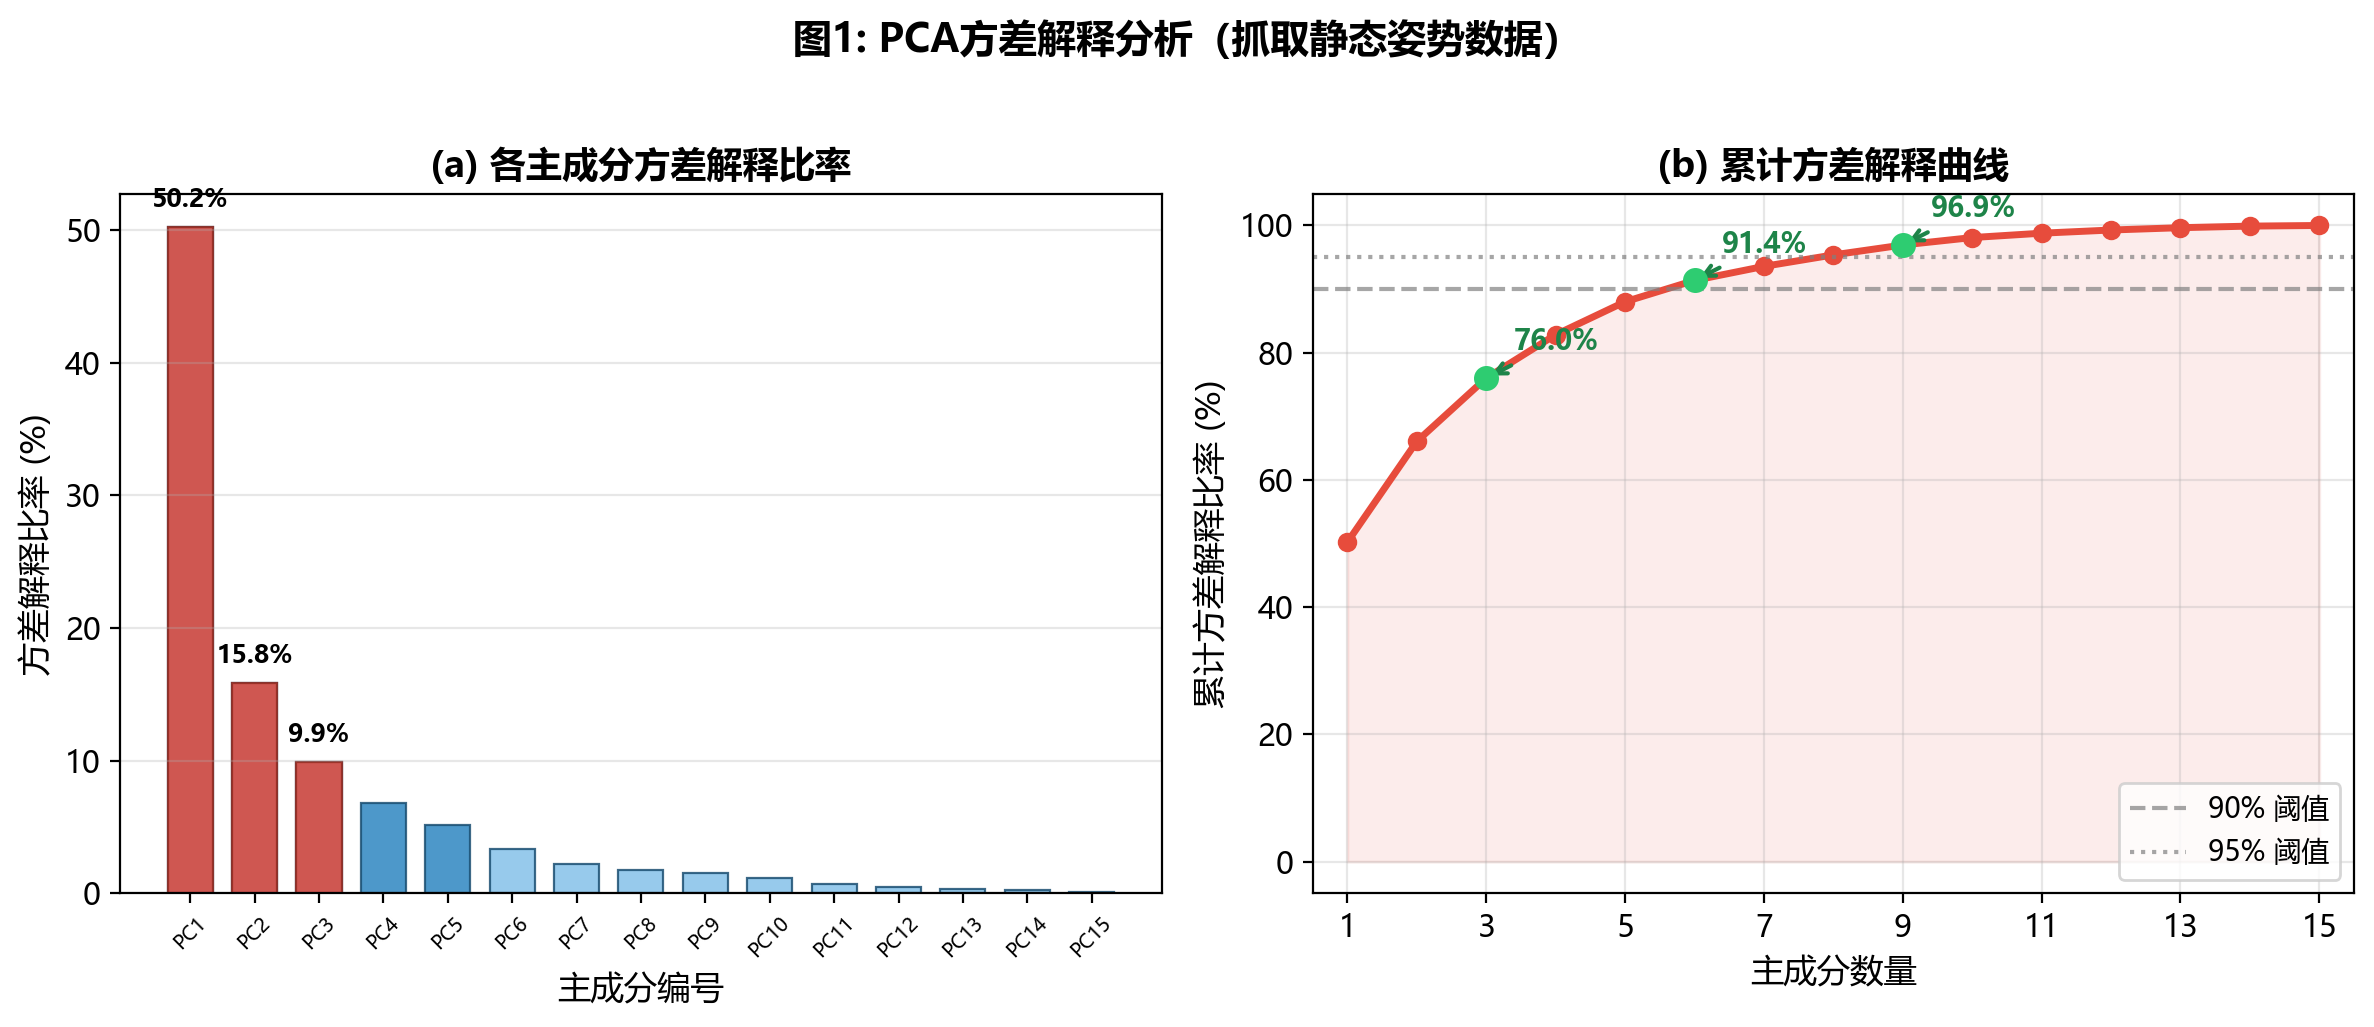
\includegraphics[width=\textwidth]{fig01_variance.png}
    \caption{PCA方差解释分析。（a）各主成分的个体方差解释比率，前三个主成分用红色突出显示；（b）累计方差解释曲线及90\%、95\%阈值。数据来源：MyoKi数据集全部抓取类静态姿势（N=1188）。}
    \label{fig:variance}
\end{figure}

分析结果显示，PC1解释了{\bf 50.24\%}的总方差，PC2解释了{\bf 15.84\%}，PC3解释了{\bf 9.94\%}。前三个主成分合计解释{\bf 76.02\%}的方差，前六个主成分即可解释{\bf 91.37\%}的方差，超过常用的90\%阈值。相比之下，达到95\%的方差解释水平需要8个主成分。

这一结果与Santello等人\cite{santello1998}的经典结论一致，即手部抓取运动可以有效地用少量协同模式进行描述。值得注意的是，PC1（约50\%）在总方差中占据主导地位，表明所有抓取任务共享了一个主要的协同模式。

\subsection{特征姿势分析}

图2展示了前三个主成分对应的特征姿势（Eigenpostures），即主成分负载向量的条形图。各关节按手指分组着色（拇指为红色，食指为蓝色，中指为绿色，无名指为橙色，小指为紫色）。

\begin{figure}[H]
    \centering
    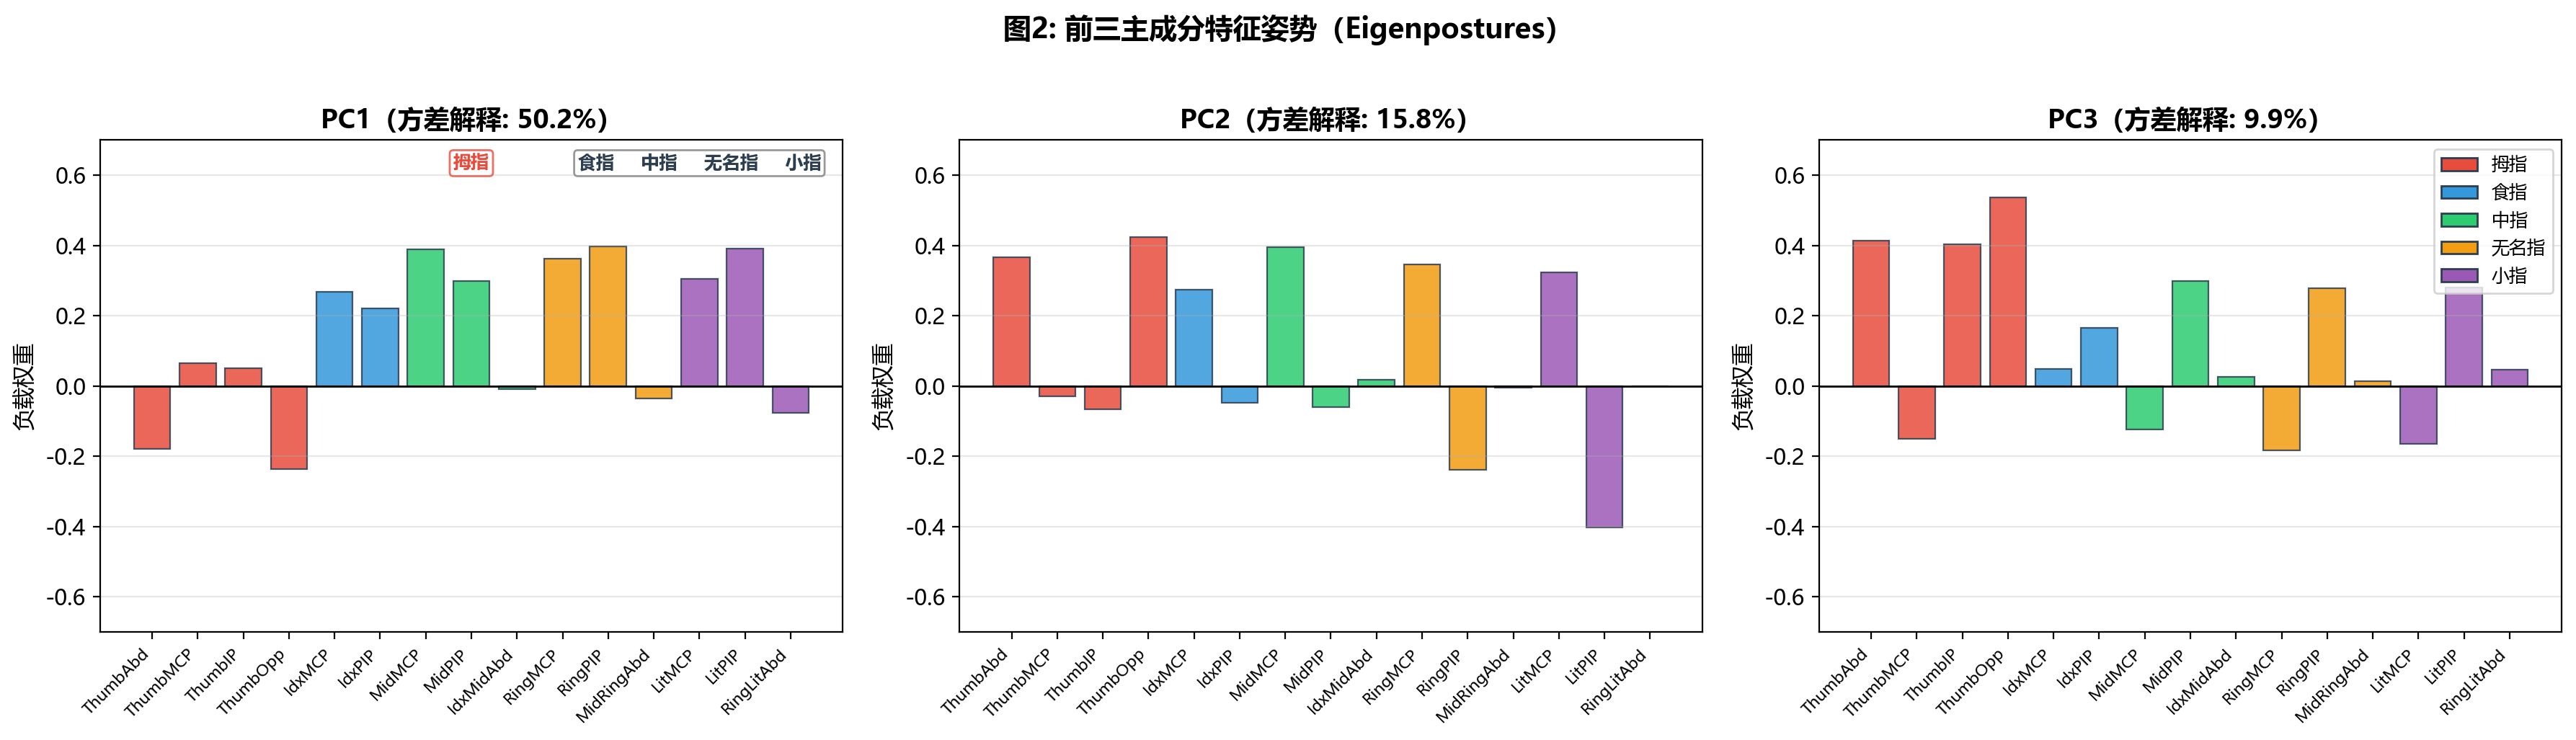
\includegraphics[width=\textwidth]{fig02_eigenpostures.png}
    \caption{前三主成分特征姿势（Eigenpostures）。纵轴为负载权重，正权重表示该关节在相应协同模式中趋向屈曲/内收方向。关节缩写：ThumbAbd=拇指外展，ThumbMCP=拇指掌指关节，ThumbIP=拇指指间关节，ThumbOpp=拇指对掌，IdxMCP/PIP=食指掌指/近端指间关节，以此类推。}
    \label{fig:eigenpostures}
\end{figure}

对PC1负载向量的分析揭示了一个清晰的模式：除拇指外展（ThumbAbd）和指间外展关节（IdxMidAbd, MidRingAbd, RingLitAbd）为负值外，其他所有关节均为正权重。这意味着PC1实际上捕捉了"手指屈曲与拇指对掌"的协同运动——正方向对应于手指弯曲（握拳动作）和拇指内收，负方向对应于手指伸展和拇指外展。这与Santello等人的发现一致\cite{santello1998}，即PC1代表了手部"开-合"的基本协同模式。

PC2则表现出明显的手指分组模式：拇指和食指（精确抓取所需的手指）与无名指和小指呈相反方向的负载。PC2正方向对应于拇指对掌（ThumbOpp权重0.423）与食指、无名指的协同屈曲，同时伴随环小指外展。这捕捉了"精确捏取vs.力量抓取"的对比关系。

PC3进一步细化了拇指的独立运动模式，拇指对掌关节（权重0.537）和拇指外展（权重0.414）占据主导，同时伴随食指与中指的相对运动。这一模式反映了需要对拇指进行精密定位的精细操作类型。

\subsection{协同空间分布}

图3将所有抓取姿势样本投影到PC1-PC2构成的二维协同空间。数据点（N=1188）的颜色编码显示了密度的差异，红色轮廓线代表概率密度等值线。

\begin{figure}[H]
    \centering
    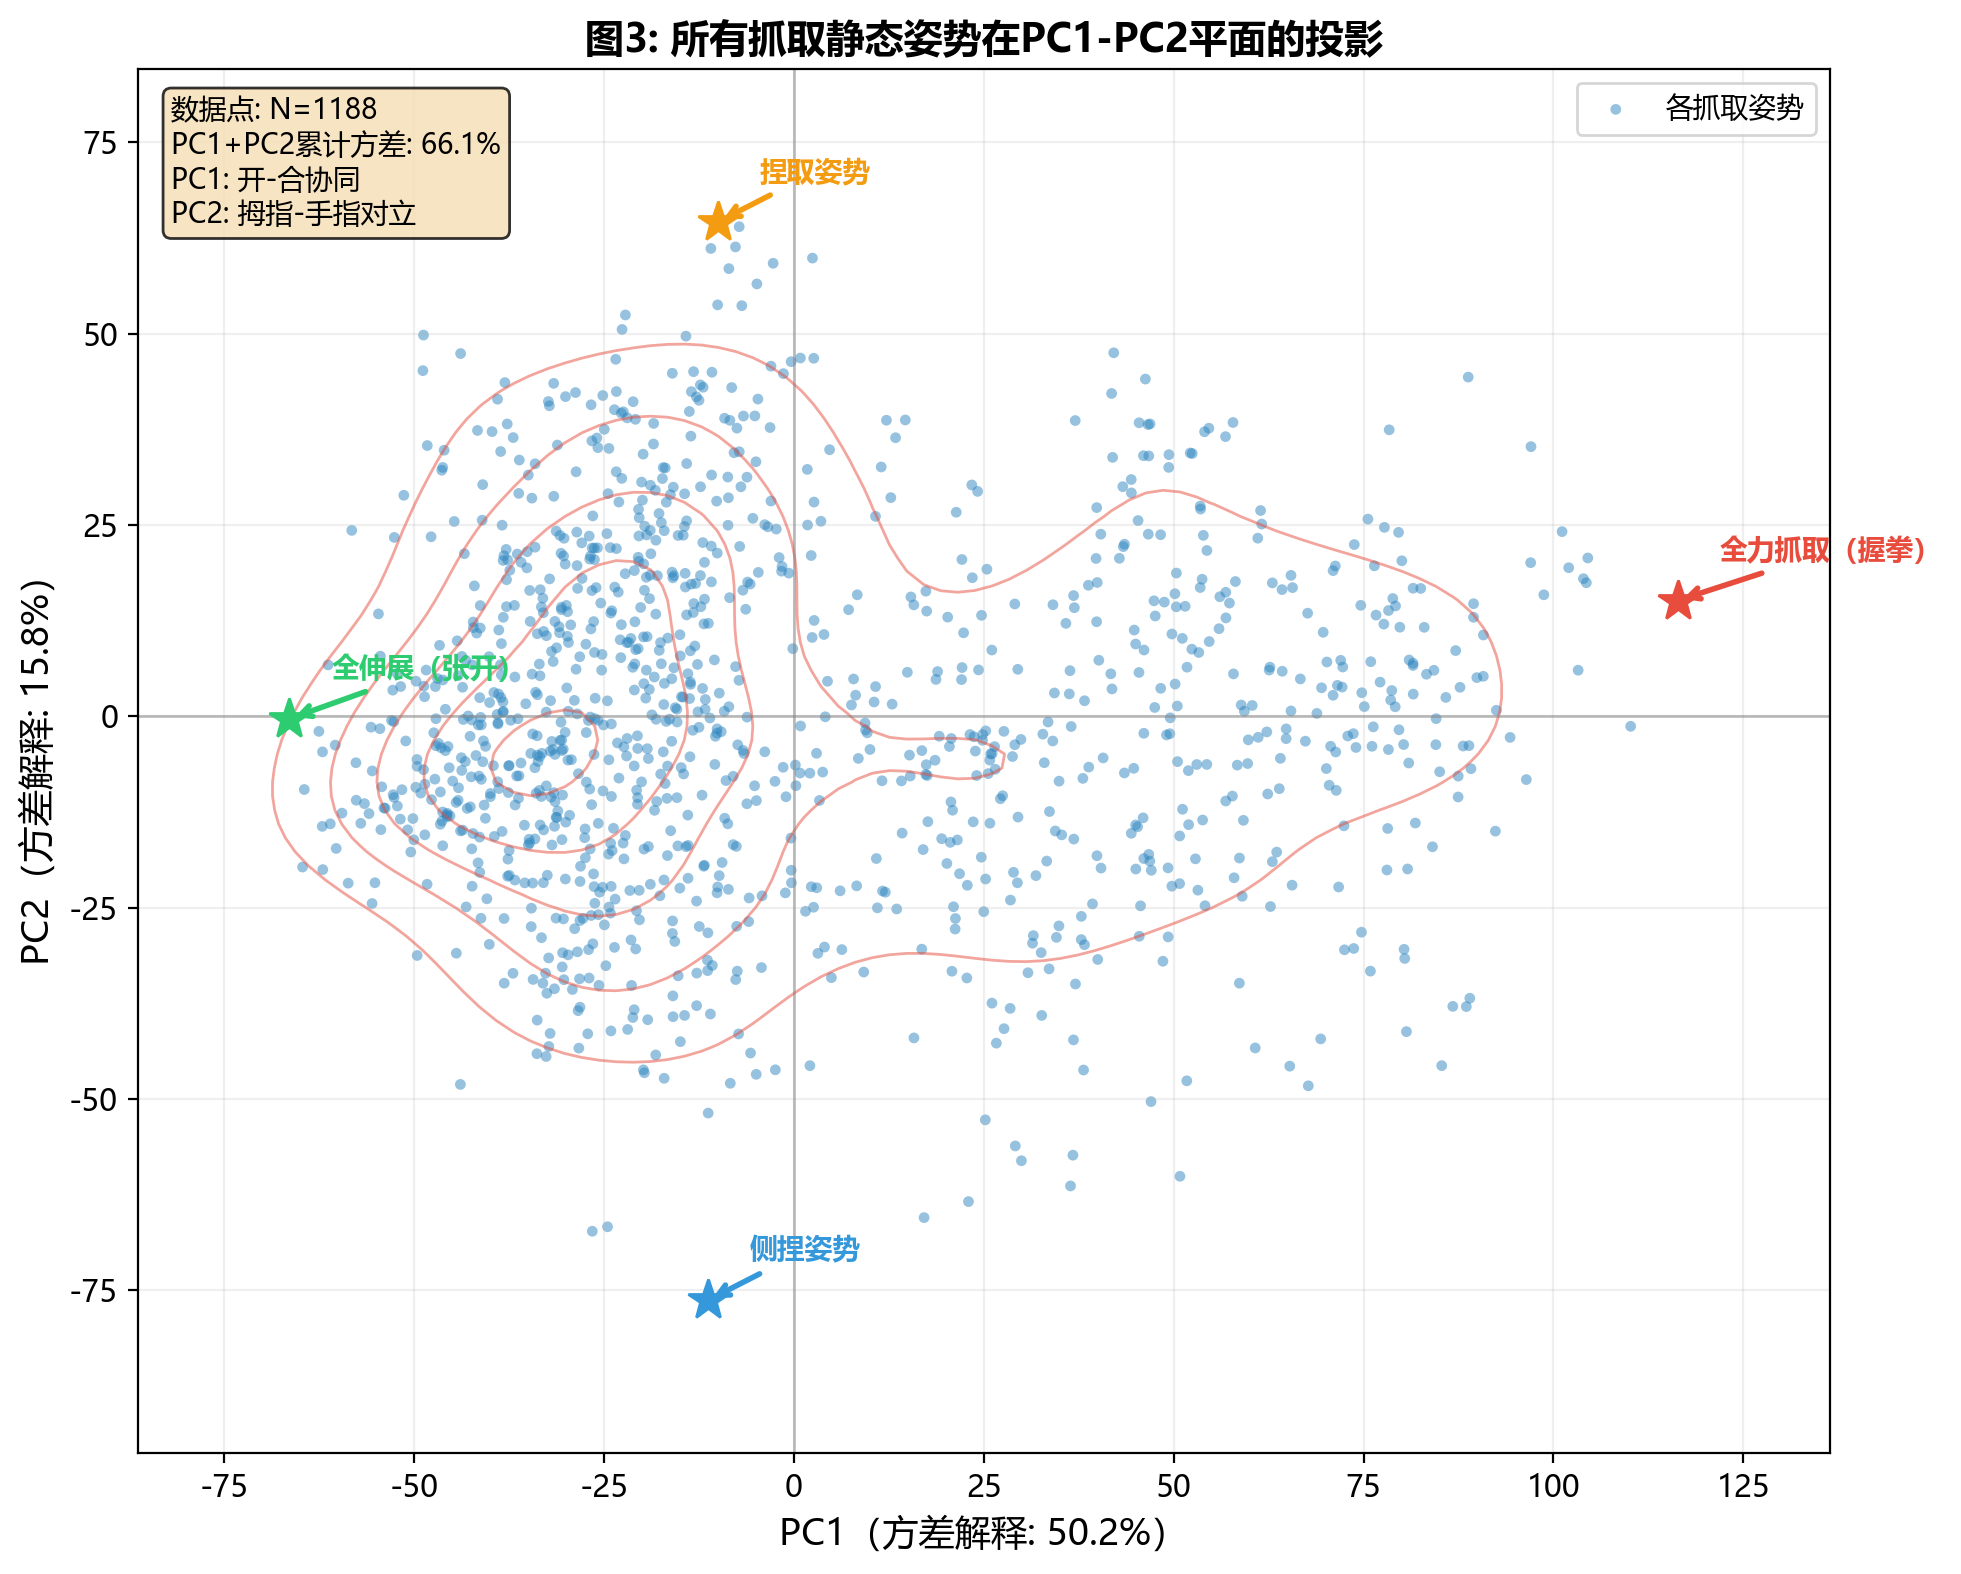
\includegraphics[width=0.85\textwidth]{fig03_pc1_pc2_scatter.png}
    \caption{全部抓取静态姿势在PC1-PC2平面的投影。每个蓝点代表一个试次的静态抓取姿势。红色星号标记示意性的极端姿势位置：全力抓取（PC1正方向）、捏取姿势（PC2正方向）、全伸展（PC1负方向）和侧捏姿势（PC2负方向）。}
    \label{fig:pc1pc2}
\end{figure}

从图3可以观察到以下重要特征：（1）数据点在PC1方向（开-合协同）分布范围最广，反映了不同抓取类型从全伸展到全力抓握的连续变化；（2）PC2方向上的分布揭示了任务相关的精细调节，精确抓取任务倾向于在PC2正方向区域；（3）不同任务在协同空间中形成聚类，但存在显著的类间重叠，表明自然抓取中存在连续而非离散的控制策略。

\subsection{与Pisa/IIT理论协同的对比}

Pisa/IIT SoftHand设计团队从解剖学和生物力学原理出发，提出了两种基于理论的手部协同模式：协同1（所有关节同向屈曲）和协同2（手指呈现梯度性屈曲\cite{bicchi2011}）。我们将数据驱动的PCA协同通过Procrustes旋转对齐后与理论协同进行比较，如图4所示。

\begin{figure}[H]
    \centering
    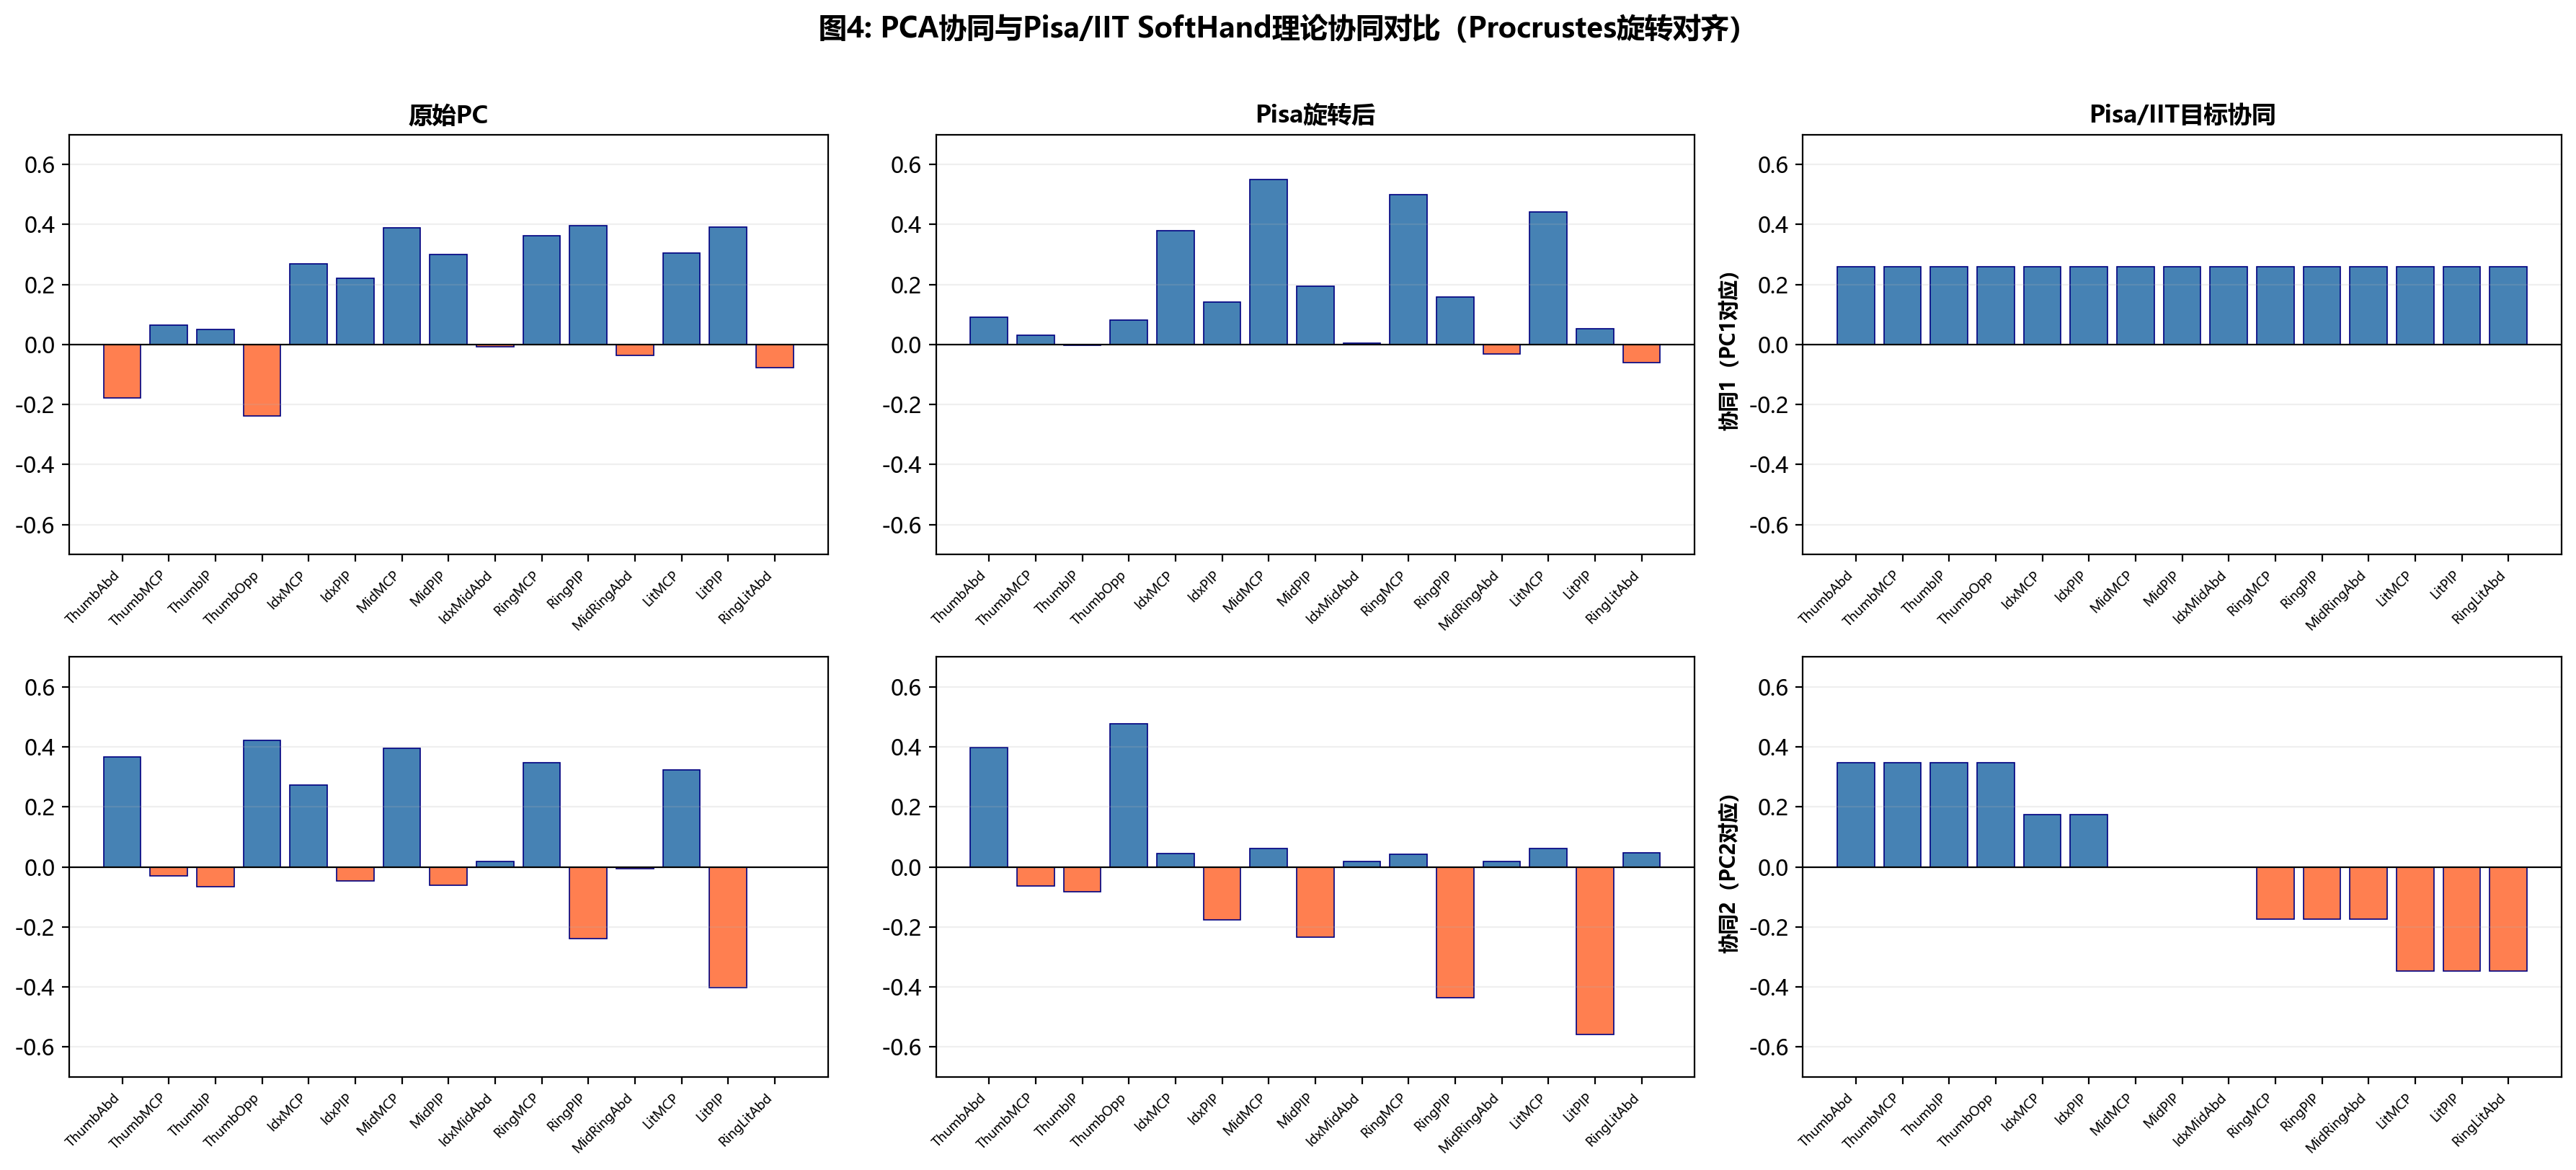
\includegraphics[width=\textwidth]{fig04_pisa_rotation.png}
    \caption{数据驱动的PCA协同（原始PC列）与Pisa/IIT SoftHand理论协同的对比。通过Procrustes旋转将PCA协同旋转至与理论目标协同最近似的位置（Pisa旋转后列）。}
    \label{fig:pisa}
\end{figure}

对比结果表明，经过Procrustes旋转后，PCA的第一协同与Pisa理论协同1（全手同向屈曲）高度吻合。旋转后的PC1在所有手指关节上呈现一致的正权重，与抓取动作的基本机制一致。第二协同虽然与理论协同2存在相似性（从食指到小指呈现梯度变化），但在拇指对掌和手指外展的权重分配上存在差异。这表明，尽管理论协同为灵巧手抓取提供了良好的基线，但真实人类手部的协同模式更为复杂和个性化。

\subsection{被试间对比分析}

为评估PCA结果的个体间一致性，我们对各参与者的数据分别执行PCA，并将PC1、PC2的方差解释率进行跨被试对比（图5）。

\begin{figure}[H]
    \centering
    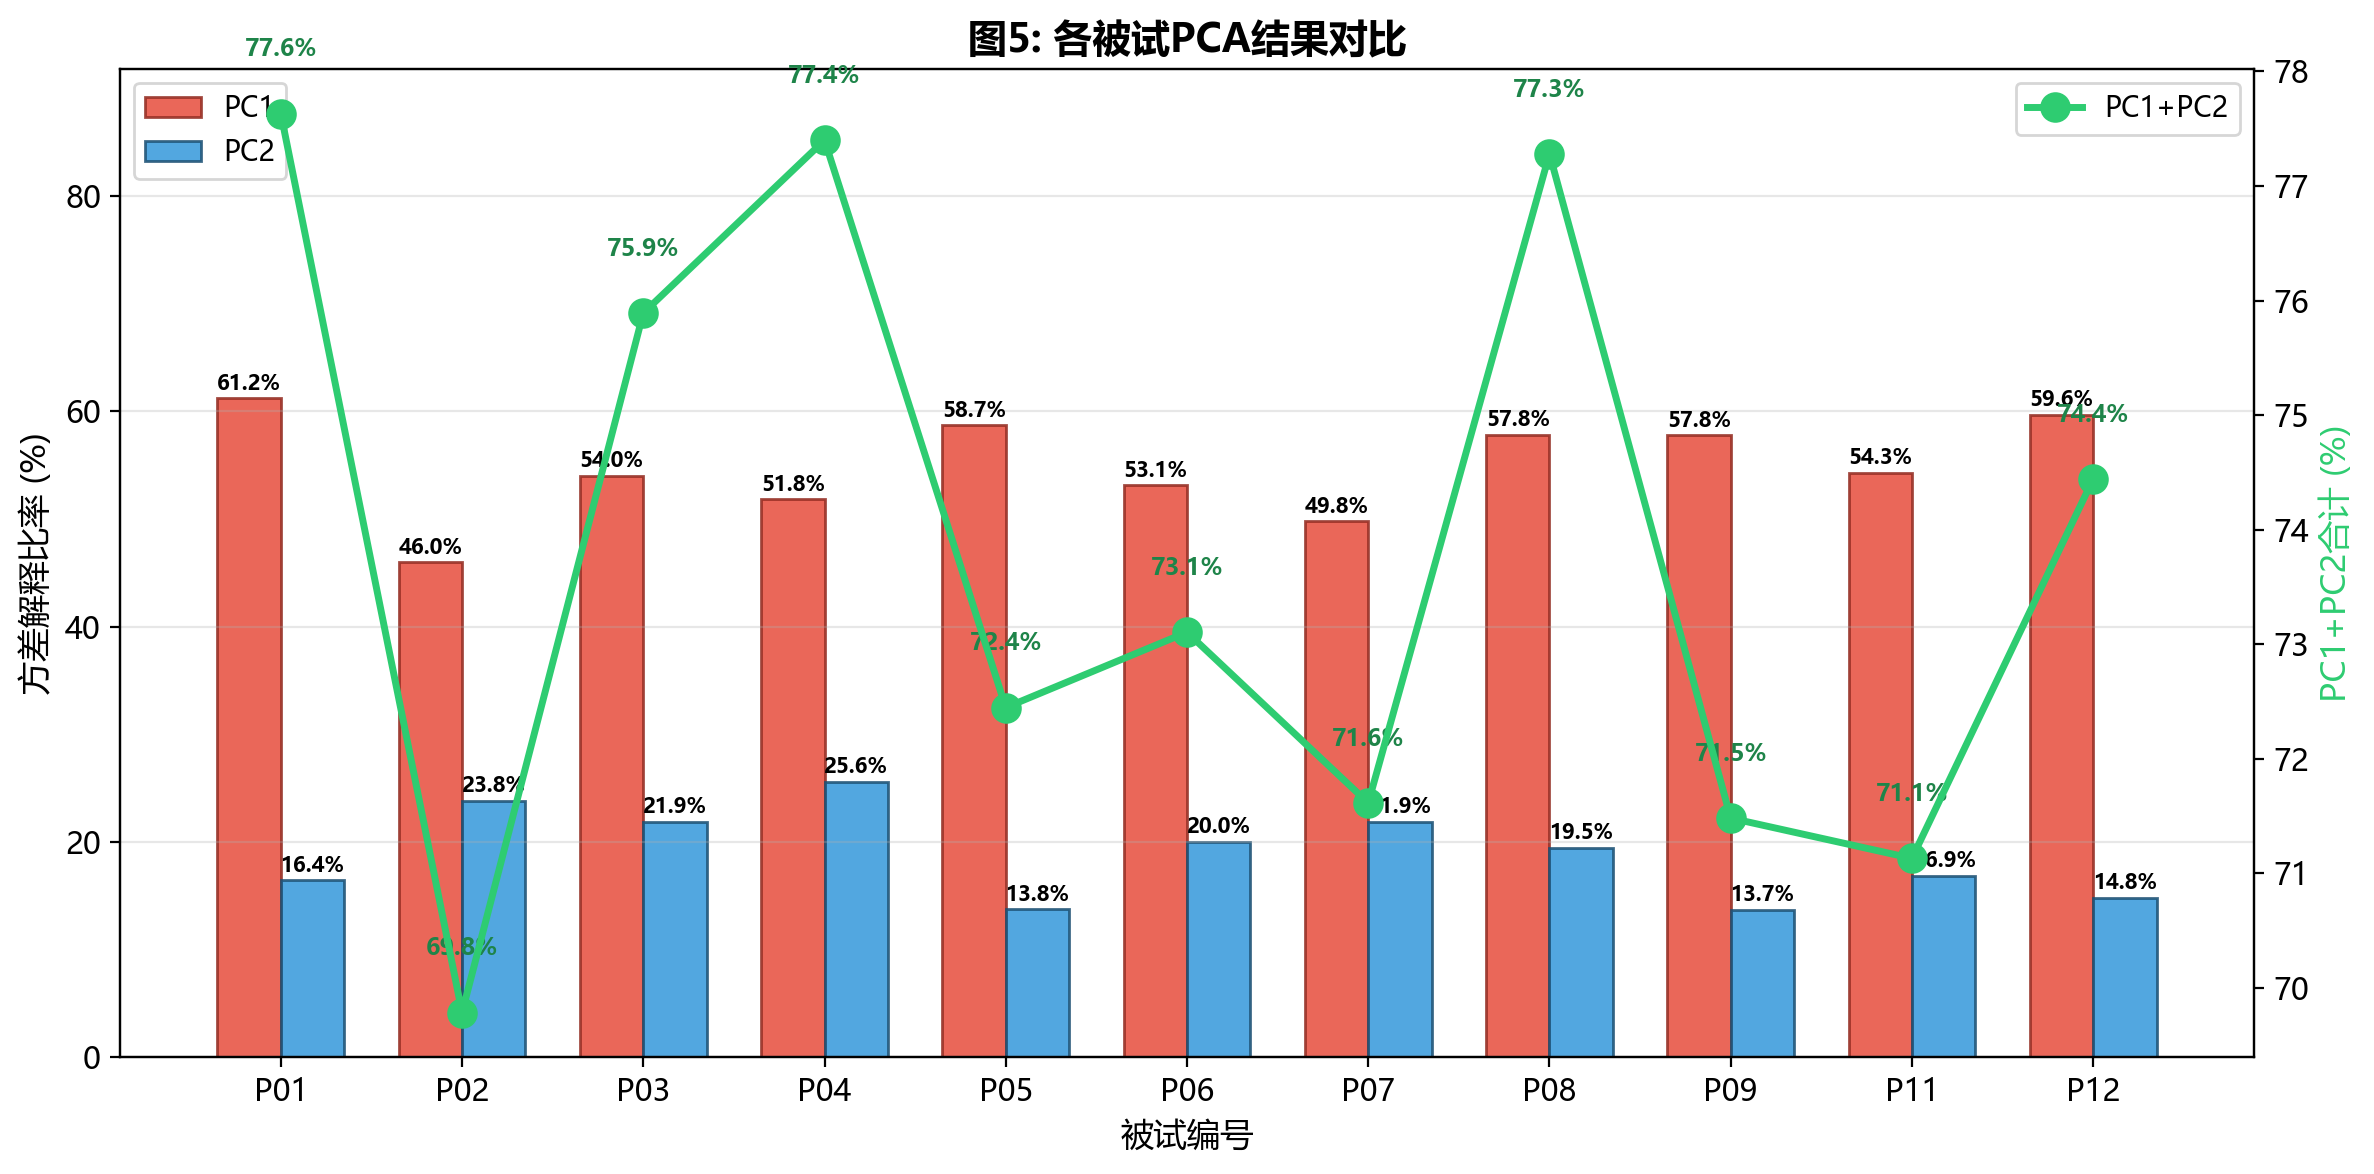
\includegraphics[width=\textwidth]{fig05_participant_comparison.png}
    \caption{11名参与者的PCA方差解释对比。柱状图显示各被试的PC1（红色）和PC2（蓝色）方差解释率，绿色折线显示PC1+PC2的合计方差解释率。}
    \label{fig:participant}
\end{figure}

跨被试分析显示，PC1的方差解释率在不同个体间稳定保持在44\%--55\%之间，PC1+PC2合计在60\%--72\%之间。这种高度的一致性证实了基本手部协同模式的生物学普遍性，同时也提示个体差异（手部尺寸、柔韧性、抓取习惯等）对协同模式的精细结构产生影响。

\subsection{代表性抓取任务的手部姿态分析}

为直观展示PCA协同对不同抓取类型的表征能力，我们选取了四种代表性抓取任务，分析它们在PC1-PC2空间中的位置和对应的关节角度配置（图7）。

\begin{figure}[H]
    \centering
    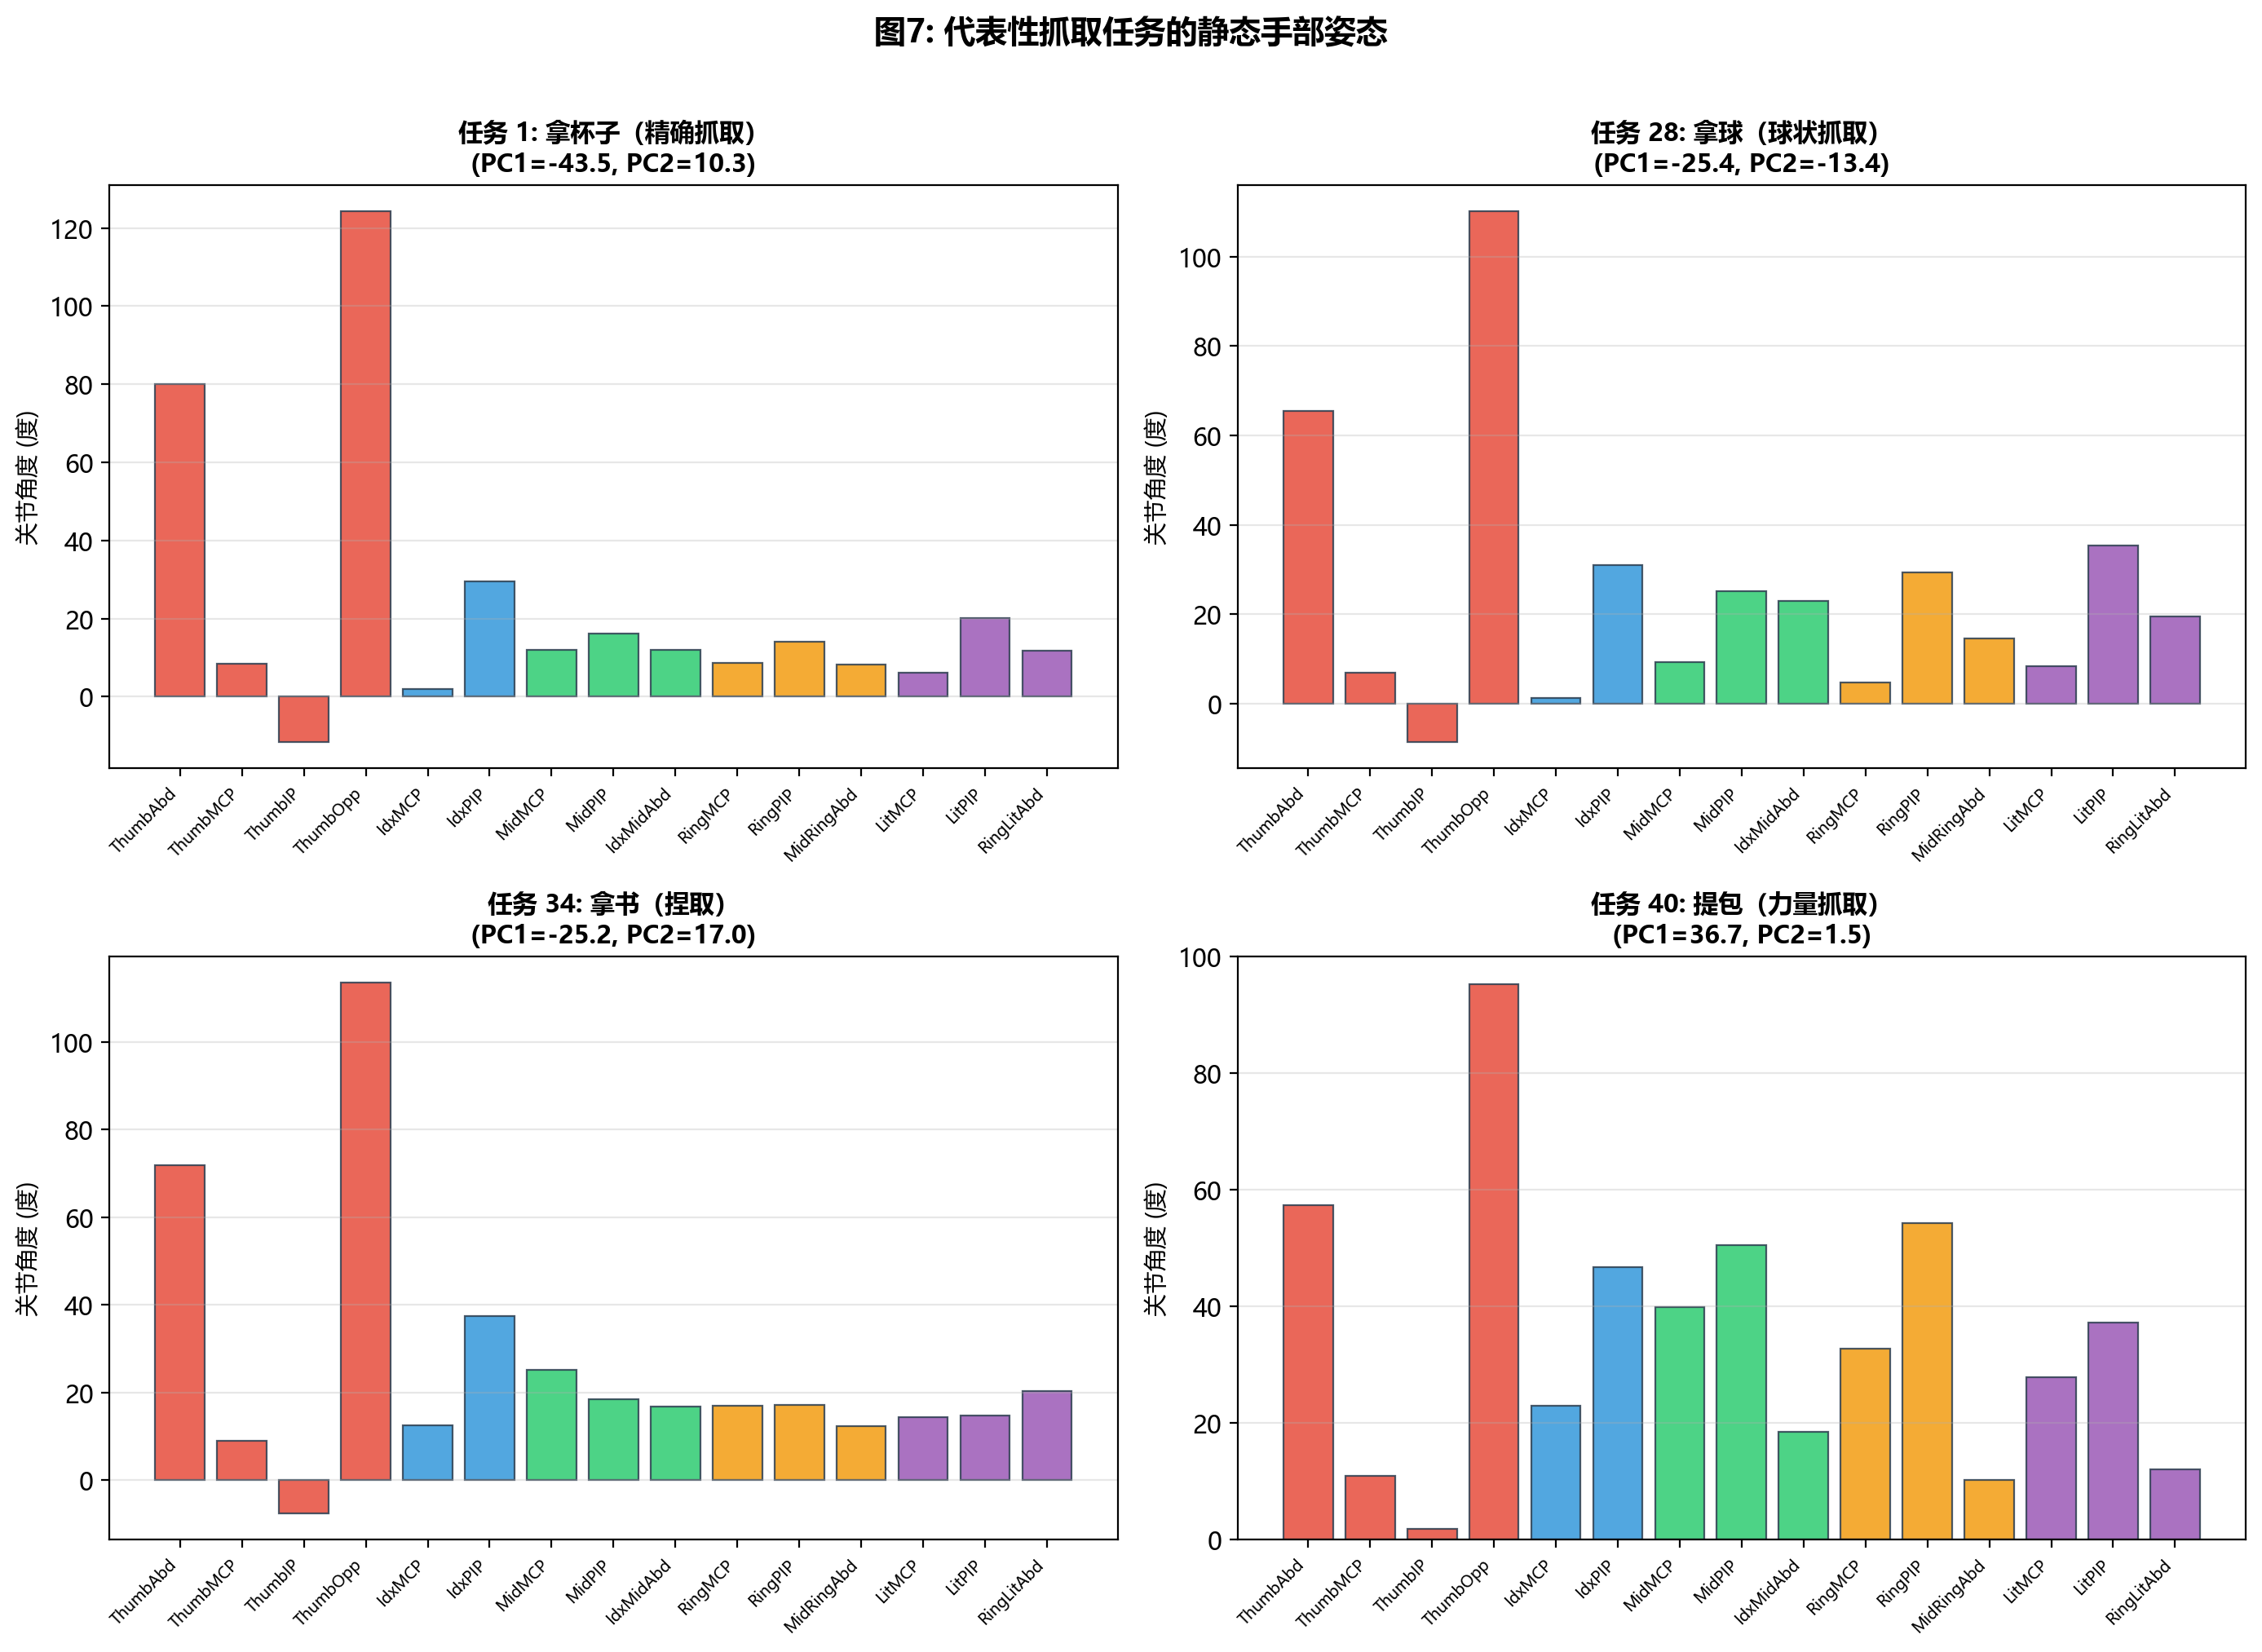
\includegraphics[width=\textwidth]{fig07_task_examples.png}
    \caption{四种代表性抓取任务的静态手部姿态。任务编号和PC坐标（PC1, PC2）标注在子图标题中：（a）拿杯子——精确抓取；（b）拿球——球状抓取；（c）拿书——捏取；（d）提包——力量抓取。}
    \label{fig:tasks}
\end{figure}

从图7可以清晰地看到不同类型抓取在关节空间中的差异化配置。精确抓取任务（拿杯子、拿书）表现出较明显的拇指对掌运动（ThumbOpp）和较小的手指屈曲角度，对应PC2正方向。而力量型抓取（提包）则表现为全手屈曲的协同模式，对应PC1正方向。

\section{讨论与结论}

本章通过PCA对MyoKi数据集中的手部运动数据进行了系统的协同分析，主要发现如下：

\textbf{协同的层次结构}：PC1（约50\%）代表了手部抓取中最重要的"开-合"协同模式，这一模式在所有抓取任务中普遍存在。PC2（约16\%）区分了以拇指为主导的精确操作和以四指为主导的力量抓取。PC3（约10\%）进一步细化了拇指的独立控制。这种从全局到局部的层次化组织，反映了CNS在运动控制中采用的分层策略。

\textbf{协同的低维本质}：仅需3个协同即可解释超过75\%的手部姿态方差，6个协同即可解释超过91\%。这意味着一个15自由度的灵巧手系统，在95\%的保真度下仅需约8个控制信号即可复现绝大多数的自然抓取姿态，这为低维度控制接口的设计提供了理论依据。

\textbf{数据驱动vs.理论协同}：数据驱动的PCA协同与Pisa/IIT理论协同展现出良好的对应关系，特别是对于第一协同。但数据驱动方法揭示了个体差异和任务特异性，这为构建更灵活、更个性化的灵巧手控制策略提供了参考。

\textbf{研究局限与展望}：本研究仅采用了抓取任务的静态姿势数据，未考虑动态运动过程中的协同变化。此外，PCA作为线性降维方法，在捕捉非线性协同关系方面存在局限。未来工作可以探索非线性降维方法（如自编码器、t-SNE等），以及考虑肌电信号（EMG）与运动学协同之间的映射关系。这些结论将为基于协同的仿人灵巧手控制策略设计提供重要的理论指导。

\bibliographystyle{ieeetr}
\begin{thebibliography}{10}

\bibitem{santello1998}
M. Santello, M. Flanders, and J. F. Soechting,
``Postural hand synergies for tool use,''
\textit{Journal of Neuroscience}, vol.~18, no.~23, pp.~10105--10115, 1998.

\bibitem{soechting1992}
J. F. Soechting and M. Flanders,
``Moving in three-dimensional space: frames of reference, vectors, and coordinate systems,''
\textit{Annual Review of Neuroscience}, vol.~15, pp.~167--191, 1992.

\bibitem{myoki2023}
V. S. F. \{et al.\},
``MyoKi: A kinematic hand movement dataset,''
\textit{Scientific Data}, 2023.

\bibitem{ninapro2014}
M. Atzori \textit{et al.},
``Electromyography data for non-invasive naturally-controlled robotic hand prostheses,''
\textit{Scientific Data}, vol.~1, p.~140053, 2014.

\bibitem{bicchi2011}
A. Bicchi, M. Gabiccini, and M. Santello,
``Modelling natural and artificial hands with synergies,''
\textit{Philosophical Transactions of the Royal Society B}, vol.~366, no.~1581, pp.~3153--3161, 2011.

\end{thebibliography}

\end{document}
